%%%%%%%%%%%%%%%%%%%%%%%%%%%%%%%%%%%%%%%%%%%%%%%%%%%%%%%%%%%%%%%%%%
%%%%%%%% ICML 2015 EXAMPLE LATEX SUBMISSION FILE %%%%%%%%%%%%%%%%%
%%%%%%%%%%%%%%%%%%%%%%%%%%%%%%%%%%%%%%%%%%%%%%%%%%%%%%%%%%%%%%%%%%

% Use the following line _only_ if you're still using LaTeX 2.09.
%\documentstyle[icml2015,epsf,natbib]{article}
% If you rely on Latex2e packages, like most moden people use this:
\documentclass{article}
\usepackage{pdflscape}
\usepackage{tabularx}
\usepackage{lipsum}
\usepackage{adjustbox}
\usepackage{amsmath,array}
\usepackage{kantlipsum}
\usepackage{float}
\usepackage{pbox}
% use Times
\usepackage{times}
% For figures
\usepackage{graphicx} % more modern
%\usepackage{epsfig} % less modern
\usepackage{subfigure} 

% For citations
\usepackage{natbib}

% For algorithms
\usepackage{algorithm}
\usepackage{algorithmic}

% As of 2011, we use the hyperref package to produce hyperlinks in the
% resulting PDF.  If this breaks your system, please commend out the
% following usepackage line and replace \usepackage{icml2015} with
% \usepackage[nohyperref]{icml2015} above.
\usepackage{hyperref}

% Packages hyperref and algorithmic misbehave sometimes.  We can fix
% this with the following command.
\newcommand{\theHalgorithm}{\arabic{algorithm}}

% Employ the following version of the ``usepackage'' statement for
% submitting the draft version of the paper for review.  This will set
% the note in the first column to ``Under review.  Do not distribute.''
%\usepackage[accepted]{icml2015} 

% Employ this version of the ``usepackage'' statement after the paper has
% been accepted, when creating the final version.  This will set the
% note in the first column to ``Proceedings of the...''
\usepackage[accepted]{icml2015}


% The \icmltitle you define below is probably too long as a header.
% Therefore, a short form for the running title is supplied here:
\icmltitlerunning{Sentiment analysis on yelp dataset}

\begin{document} 





\twocolumn[
\icmltitle{Sentiment analysis on yelp dataset}


% It is OKAY to include author information, even for blind
% submissions: the style file will automatically remove it for you
% unless you've provided the [accepted] option to the icml2015
% package.
\icmlauthor{Naga Venkata Sai Indubhaskar Jupudi}{njupudi@ucsc.edu}
\icmlauthor{Trivikram Bollempalli}{tbollemp@ucsc.edu}
\icmlauthor{Chandrahas Jagadish Ramalad}{cjagadis@ucsc.edu}
\icmlauthor{Karthikeyan Subramanian}{ksubram1@ucsc.edu}\\
\\
GitHub Link : \url{https://github.com/jupudibhaskar967/CMPS-242-Project.git}

% You may provide any keywords that you 
% find helpful for describing your paper; these are used to populate 
% the "keywords" metadata in the PDF but will not be shown in the document
\icmlkeywords{boring formatting information, machine learning, ICML}
\vskip 0.3in
]




%%\begin{abstract} 
 
%%\end{abstract}  

%%%%%%%%%%%%%%%%%%%%%%%%%%%%%%%%%%%%%%%%%%%%%%%%%%%%%%%%%%%%%%%%%%%%%%%%%%%%%%%%%%%%%%%%%%%%%%%%%%%%%%%%%%%%%%%%%%%%%%%%

\section{Problem statement}
In this project, we aim to perform sentiment analysis on the yelp dataset. Using reviews and rating data for training, given a new review we classify it as a positive/negative review (binary) and also predict the rating (multiclass). A review is considered positive if it has received a rating of 4 or 5 and negative if it's rating is 1 or 2. The classification problem can be solved by a set of algorithms. Every algorithm has its own advantages and disadvantages in terms of accuracy and model complexity. 

For example, naive Bayes classifier is faster to compute than logistic regression classifier for huge datasets. But the disadvantage with the former is that it assumes the features are independent where as the latter has no such assumptions which can lead to better precdiction. Our work mainly concentrates on implementing these two classifiers and techniques to improve their performance. We have adopted multi-processing for feature extraction to make it considerably faster. We have implemented stochastic gradient descent as an optimizer for logistic regression. We have also implemented Naive Bayes classifier as a baseline to compare our results from logistic regression. Finally, we contrast these algorithms based on time taken for execution and performance metrics like accuracy, precision and recall.


%%%%%%%%%%%%%%%%%%%%%%%%%%%%%%%%%%%%%%%%%%%%%%%%%%%%%%%%%%%%%%%%%%%%%%%%%%%%%%%%%%%%%%%%%%%%%%%%%%%%%%%%%%%%%%%%%%%%%%%%

\section{Feature Extraction}

We have extracted the features for respective algorithms using our own constraints instead of using countvectorizer(). This is because countvectorizer() is throwing a run-time exception for a large dataset (\textgreater300k reviews).

\subsection{Binary classification}
For logistic regression, we need to form a count vector from bag of words. To generate this, first we extracted 4/5 th of our total dataset (which is our training data) and extracted the words and their respective counts into a dictionary. We make sure none of the stop words are added to this dictionary. We got these stop words from nltk corpus. Further, we removed all the punctuation and numerical characters from the words before adding them to the dictionary. 


We then apply three constraints on this dictionary to form a bag of words (BOW). One, if a word occurs for 'x' times in all the positive reviews then it's added into BOW only if it occurs for less than 4/10 th times in all the negative reviews and vice-versa. Second, total word count for a specific word should be more than 14 over all the reviews. Third, we add the word into BOW only if it's length is greater than 2. We arrived at these numerical values after tuning the algorithm for high accuracy and being memory efficient. 


The intuition behind this is, if a word has approximately equal count over both positive and negative reviews will have less impact on the decision rule. Also removing less frequent words (\textless10 or so which might be a typing mistake) is similar to considering top-k frequent words. All single and double character words are considered as stop words.

After obtaining the BOW, we formed count vector 'x', using multi-processing (as it is both cpu intensive) to make it faster as each review can be formed into a count vector indepedently of each other. This is acheived using multiprocessing.Pool library in python. The pool.map\_async() to  all the individual vectors into a single matrix. 

For naive Bayes algorithm, we used all the words in the initial dictionary without using any constraints as there is no requirement for us to form the count vector as we did in logistic regression and the computation is way faster because of the assumption that features are independent of each other. 


\subsection{Multiclass classification}

For multiclass logistic regression, we did not use the same constriants as we did earlier for the binary case. Instead, we have selected most frequent 10k words from the dictionary after extracting the reviews. Later, we have formed the count vector 'x' in the same way as above using multi-processing. We did the same thing for Naive Bayes algorithm, as we did in the binary classification.

\subsection{Most distinctive features}
The following tables shows a set of disctinctive features which shows a glimpse of our dataset.
\begin{table}[H]
\caption{Distinctive words of the dataset.}
\vspace{1mm}
\label{sample-table}
\begin{small}
\begin{sc}
\begin{adjustbox}{width=0.5\textwidth}
\begin{tabular}{|l|l|}
\hline
Class &  Disctinctive words\\
\hline
Positive  &  \pbox{20cm}{\vspace{1mm}satisfying, heavenly, treats, sweetness, heaven, \\incredible, gem, addicted, complement, great,\\ cheers, awesome, cream, candies, concoction\vspace{1mm}}\\
\hline
Negative  &  \pbox{20cm}{\vspace{1mm}uninterested, roaches, blatant, dispute, kills,\\ annoyed, unethical, plague, trash,creepy,\\ flavorless, disrespect, unsalted, manager, insulted\vspace{1mm}}\\
\hline
\end{tabular}
\end{adjustbox}
\end{sc}
\end{small}
\end{table}

%%%%%%%%%%%%%%%%%%%%%%%%%%%%%%%%%%%%%%%%%%%%%%%%%%%%%%%%%%%%%%%%%%%%%%%%%%%%%%%%%%%%%%%%%%%%%%%%%%%%%%%%%%%%%%%%%%%%%%%%

\section{Model Formulation}
From Feature Engineering, we get input data and its labels. we will use this to train our logistic regression algorithm. We have implemented both logistic regression for two classes and also multi-class logistic regression.
\subsection{Binary Logistic Regression}


\begin{equation*}
P(C_{1}|X) = \vspace{10mm}   \frac{p(X|C_{1}).p(C_{1})}{p(X|C_{1}).p(C_{1}) + p(X|C_{2}).p(C_{2})}
\end{equation*}



The probability for the first class is given by 
\begin{equation*}
P(C_{1}|X) = y(x)  = \sigma(W\textsuperscript{T}X + b) 
\end{equation*}
The likelihood is given as 
\begin{equation*}
P(t|W) = \prod\limits_{n=1}^N (y_{n})^{t_{n}}(1-y_{n})^{1- t_{n}}
\end{equation*}

The cost function is 
\begin{equation*}
E(w) = -ln  p(t|W) = -\sum\limits_{n=1}^N t_{n}ln(y_{n}) + (1-t_{n})ln(1-y_{n})
\end{equation*}

Gradient is calculated as follows
\begin{equation*}
\nabla E(w) = \sum\limits_{n=1}^N (y_{n} - t_{n}) \phi_{n}
\end{equation*}



\subsection{Multiclass Logistic regression}
The probability of a class in logistic regression with multiple
classes is given by:
\begin{equation*}
P(C_{k}|\boldsymbol{X}) =  \frac{p(\boldsymbol{X}|C_{k}).p(C_{k})}{\sum\limits_{j}p(\boldsymbol{X}|C_{j}).p(C_{j})}
\end{equation*}
that is,,
\begin{equation*}
P(C_{k}|\boldsymbol{X}) =  y_{k}(\phi) = \frac{exp(a_{k})}{\sum\limits_{j} exp(a_{j})}
\end{equation*}

where 

\begin{equation*}
a_{k} = ln p(\boldsymbol{X}|C_{k}) + ln  p(C_{k})
\end{equation*}

We estimated the parameters using Maximum Log Likelihood
estimation. For N data points, the likelihood function is

\begin{equation*}
p(T|\boldsymbol{w_{1},..,w_{k}}) = \prod\limits_{n=1}^N \prod\limits_{k=1}^K p(C_{k}|\phi_{n})^{t_{nk}} = \prod\limits_{n=1}^N \prod\limits_{k=1}^K y_{nk}^{t_{nk}}
\end{equation*}

where,

\begin{equation*}
y_{nk} = y_k(\phi_{n})
\end{equation*}
Taking log on both sides
and negation of it, we get the below negative log likelihood
function:

\begin{equation*}
E (\boldsymbol{w_{1}},..., \boldsymbol{w_{k}} ) = -ln p(T|\boldsymbol{w_{1}},...,\boldsymbol{w_{k}}) = - \sum\limits_{n=1}^N \sum\limits_{k=1}^K t_{nk} ln y_{nk}
\end{equation*}

E(w) is our cost
function which we want to minimize to estimate W parameters.
The gradient for the cost function is given by


\begin{equation*}
\nabla E (\boldsymbol{w_{1}},..., \boldsymbol{w_{k}} ) = \sum\limits_{n=1}^N(y_{nj} - t_{nj}) \phi_{n}
\end{equation*}





\subsection{Optimization techniques}
We used fmin\_l\_bfgs\_b and stochastic gradient descent to minimize the cost function and obtain weight vector W. fmin\_l\_bfgs\_b is from scipy.optimize module in python. It uses the gradient that we calculated above in minimizing the cost function.

We also implemented Stochastic Gradient Descent(SGD) because the other optimization takes considerably longer time to execute. The advantage with SGD is that we can control the number of iterations and learning rate alpha there by controlling the total runtime of the algorithm. We have tested this with a dataset size of 300k and the execution completed in around 75 minutes. In gradient descent, we find gradient for the entire training dataset and then update W using W = W - alpha*gradient(w,x,y). Here alpha is the learning rate, W is the weight vector, x,y are training data. At each step, gradient descent updates W, trying to minimize the cost. This is true as long as we choose proper alpha. Gradient descent converges close to global minimum since the cost function is convex. In SGD, W is updated by finding gradient for each sample. We can also find gradient over a batch of training data which is a compromise between the two extremes. Finding gradient over a batch will increase the performance compared to a single sample because we can use vectorization to make it faster. We have implemented SGD in this way where you can specify batch size.
%%%%%%%%%%%%%%%%%%%%%%%%%%%%%%%%%%%%%%%%%%%%%%%%%%%%%%%%%%%%%%%%%%%%%%%%%%%%%%%%%%%%%%%%%%%%%%%%%%%%%%%%%%%%%%%%%%%%%%%%
\section{Evaluation}

We performed all our experiments on a server that has 24 physical cores (with hyperthreading 2) and 128GB of DRAM. We are testing our binary and multinomial logistic regression algorithms on yelp dataset. We are using three metrics viz., Accuracy, Precision, Recall to evaluate these algorithms. These three metrics are calculated as follows.


Accuracy = (number of correctly classified test cases) / (total number of test cases) 


Precision = (true positives) / (true positives + false positives)


Recall =  (true positives) / (true positives + false negatives)


We also compare the performance of our logistic regression algorithm with naive bayes approach and discuss tradeoffs. We compare the performance of logistic regression when fmin\_l\_bfgs\_b() and Stochastic Gradient Descent are used as optimizers.

%%%%%%%%%%%%%%%%%%%%%%%%%%%%%%%%%%%%%%%%%%%%%%%%%%%%%%%%%%%%%%%%%%%%%%%%%%%%%%%%%%%%%%%%%%%%%%%%%%%%%%%%%%%%%%%%%%%%%%%%
\section{Results}


\subsection{Effect of parallelism}
We implemented multi-processing to compute the feature vector in order to make it faster as it is a cpu intensive operation. The following table is drawn to illustrate the time taken for extracting the features from 100k and 50k reviews. With parallelism, we are able to achieve 10x speed in time taken for execution.


\begin{table}[H]
\caption{Execution time for extraction of features in Logistic regression classifier.}
\label{sample-table}
\begin{center}
\begin{small}
\begin{sc}
\begin{tabular}{lllll}
\hline
Parallelism & Size & Features & Time \\
\hline
No  & 100k & 9049 & 65m36.271s \\
No  & 50k & 5323 & 18m32.441s \\
Yes  & 100k & 9049 & 7m8.291s \\
Yes  & 50k & 5323 & 2m36.947s \\
\hline
\end{tabular}
\end{sc}
\end{small}
\end{center}
\end{table}


As explained earlier, we have designed our own feature extraction algorithm because the built-in function countvectorizer() is throwing a run-time exception for a huge dataset which is beyond 300k reviews.


\begin{table}[H]
\caption{Parallelism vs countvectorizer()}
\label{sample-table}
\begin{center}
\begin{small}
\begin{sc}
\begin{tabular}{lllll}
\hline
Method & Features & Time \\
\hline
Parallel  & 17083 & 42m27.394s \\
countvectorizer  & 10k & Run-Time error \\
\hline
\end{tabular}
\end{sc}
\end{small}
\end{center}
\end{table}


\subsection{Binary classification}
\subsubsection{fmin\_l\_bfgs\_b vs stochastic gradient descent}
We have extracted 50k reviews out of which we used 40K reviews for training and 10k reviews for testing. The total number of features are 5437. 
Figure 1 illustrates the performance statistics of logistic regression classifier with fmin\_l\_bfgs\_b vs stochastic gradient descent optimization. As it is evident from the figure, the former optimization is 16 times slower than the latter and also good accuracy can be obtained by carefully varying the alpha parameter in SGD. Label1 represents postive review (rating greater than 3) and label2 represents negative review (rating less than 3).

\begin{figure}[H]
  \caption{fmin\_l\_bfgs\_b vs stochastic gradient descent}
  \centering
    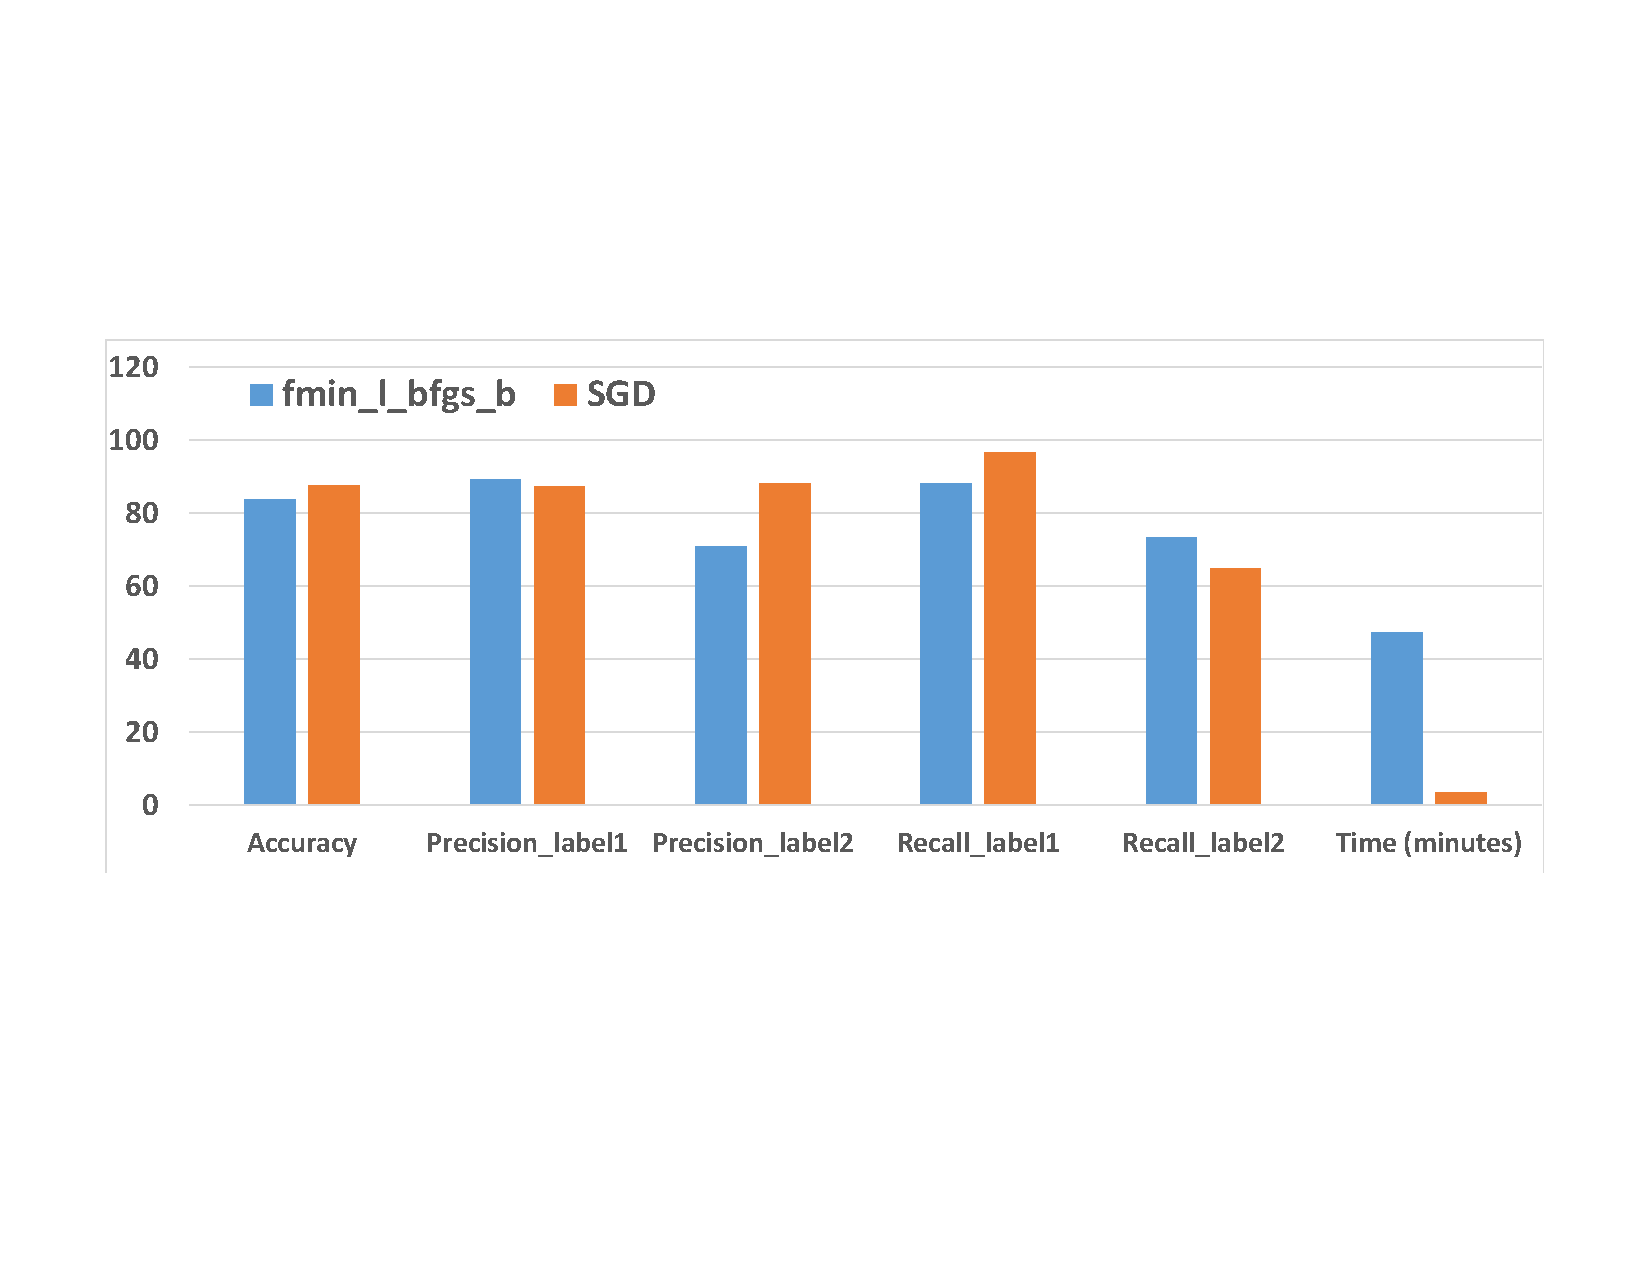
\includegraphics[width=0.5\textwidth,height=3.5cm]{newtemp}
\end{figure}


\subsubsection{stochastic gradient descent vs naive Bayes}
Here, we have extracted 100k reviews out of which we used 80k reviews for training and 20k for testing. The total number of features for logistic regression are 8871. Figure 2 illustrates the performance statistics of logistic regression classifier with SGD vs naive Bayes classifier.  As it is evident from the figure that naive Bayes classifier is faster than SGD optimized logistic regression but the accuracy obtained is less.
\begin{figure}[H]
  \caption{stochastic gradient descent vs Naive Bayes classifier}
  \centering
    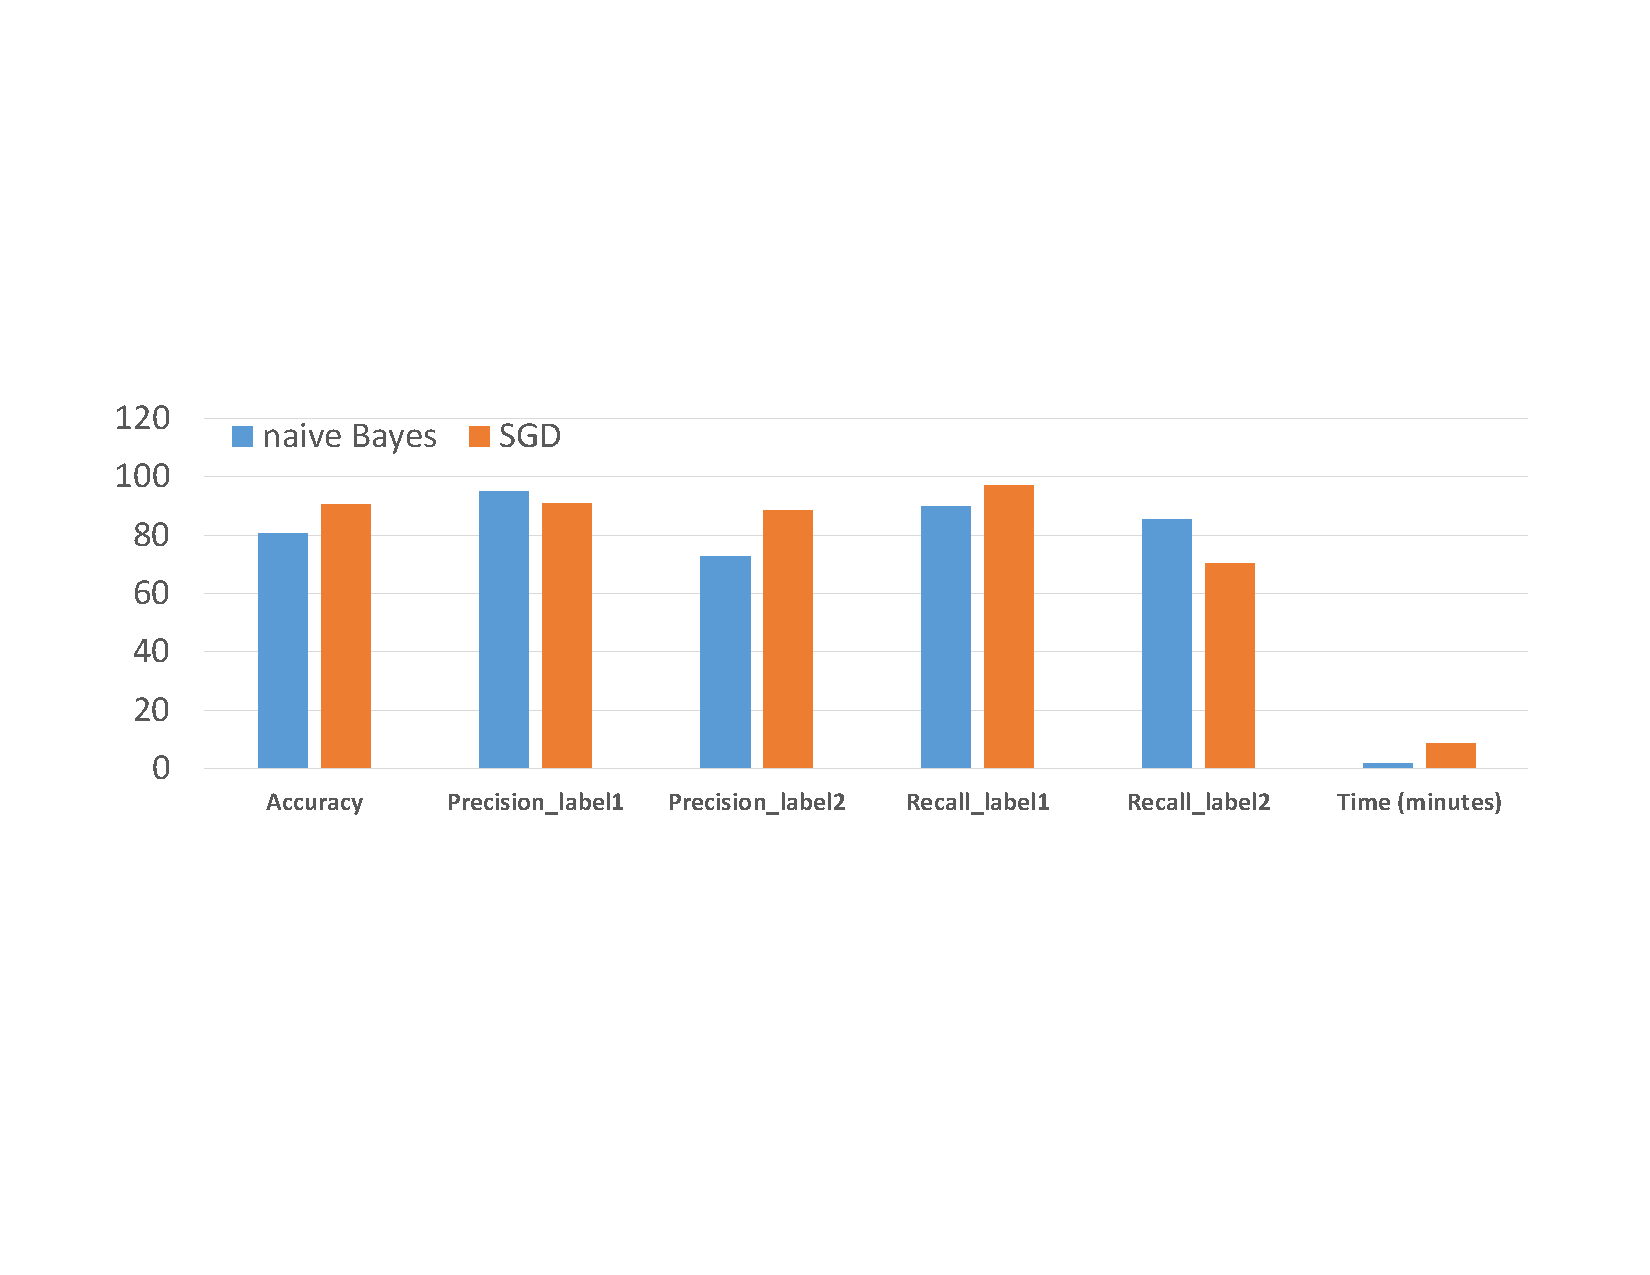
\includegraphics[width=0.5\textwidth]{sgdvsbayes}
\end{figure}



\subsection{Multiclass classification}
We have extracted 100k reviews out of which we used 80k reviews for training and 20k for testing. The total number of features for logistic regression are 10103 using top-10000 frequent words. Figure 3 illustrates the performance statistics of logistic regression classifier with SGD vs naive Bayes classifier for multi-class classification.  As it is evident from the figure that naive Bayes classifier is faster than SGD optimized logistic regression but the accuracy obtained is less.

\begin{figure}[H]
  \caption{stochastic gradient descent vs Naive Bayes classifier}
  \centering
    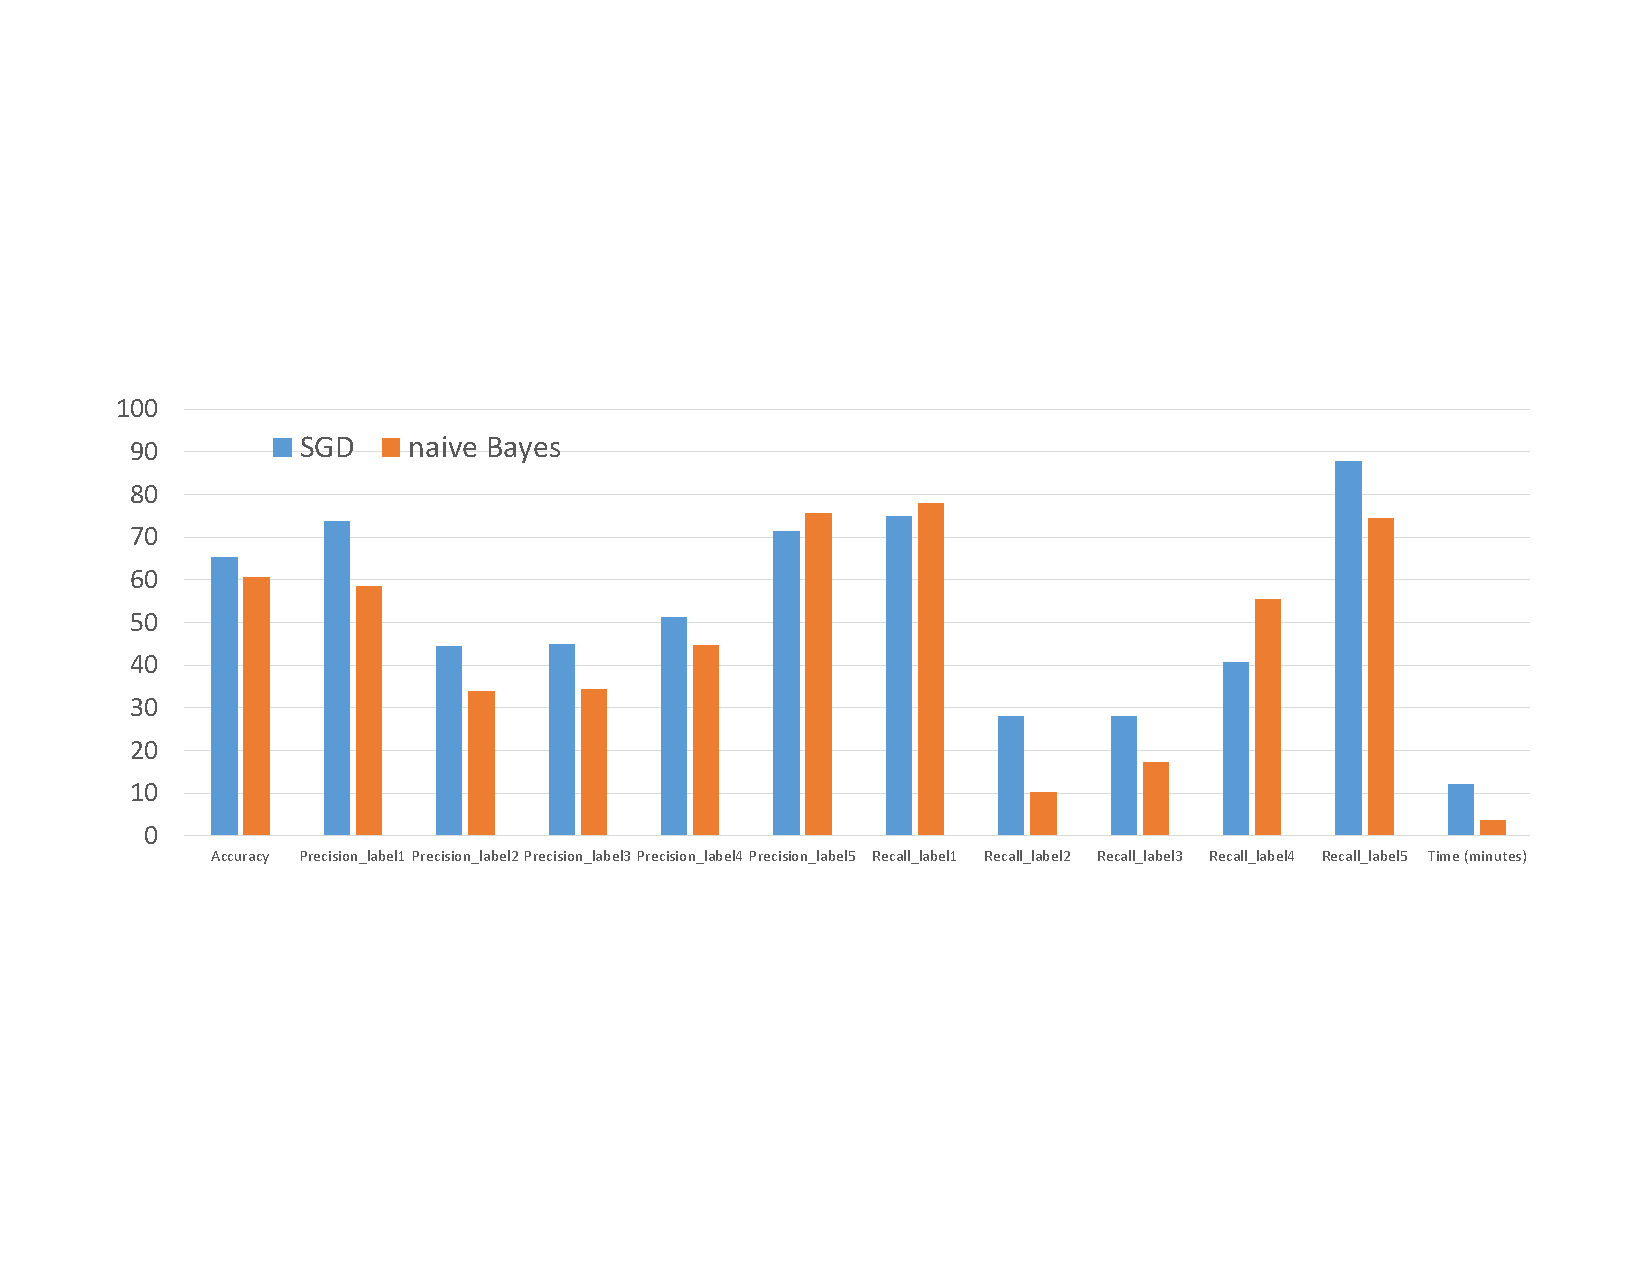
\includegraphics[width=0.5\textwidth]{cropped_Book2}
\end{figure}



%%%%%%%%%%%%%%%%%%%%%%%%%%%%%%%%%%%%%%%%%%%%%%%%%%%%%%%%%%%%%%%%%%%%%%%%%%%%%%%%%%%%%%%%%%%%%%%%%%%%%%%%%%%%%%%%%%%%%%%%

\section{Conclusion}
We have performed Sentiment Analysis using logistic regression and compared the performance with naive Bayes approach. We have also predicted rating based on the reviews using multiclass logistic regression and compared with multinomial naive Bayes.


The advantages of logistic regression classifier is that it does not have any assumptions on the features or the underlying data resulting in a better accuracy, precision and recall. But the downside of this classifier is it requires powerful machines (with advanced cpus’ and more memory) to compute the feature vector.


The advantages of naive Bayes classifier is that the time taken for execution is considerably faster when compared to logistic regression classifier and it do not require any powerful  specifications of the machine. But the downside is that it assumes that features are independent of each other which sometimes results in a poor accuracy when the data has highly correlated features


So we recommend Logistic regression if accuracy, precision or recall is an important criteria compared to the time taken for training. If the training data is not updated regularly, then we recommend logistic regression, as ‘W’ can be calculated once and used for predictions. We recommend naive Bayes, when the algorithm needs to be trained faster and accuracy can be compromised a little. We also recommend naive bayes, if the features are known to be independent of each other. We also suggest stochastic gradient descent rather than fmin\_l\_bfgs\_b for optimization in Logistic Regression.

%%%%%%%%%%%%%%%%%%%%%%%%%%%%%%%%%%%%%%%%%%%%%%%%%%%%%%%%%%%%%%%%%%%%%%%%%%%%%%%%%%%%%%%%%%%%%%%%%%%%%%%%%%%%%%%%%%%%%%%%
% In the unusual situation where you want a paper to appear in the
% references without citing it in the main text, use \nocite


\nocite{chameleon}
\nocite{Bryan}
\nocite{python}
\nocite{log}
\nocite{nb}
\bibliography{example_paper}
\bibliographystyle{icml2015}


%%%%%%%%%%%%%%%%%%%%%%%%%%%%%%%%%%%%%%%%%%%%%%%%%%%%%%%%%%%%%%%%%%%%%%%%%%%%%%%%%%%%%%%%%%%%%%%%%%%%%%%%%%%%%%%%%%%%%%%%


\end{document} 


% This document was modified from the file originally made available by
% Pat Langley and Andrea Danyluk for ICML-2K. This version was
% created by Lise Getoor and Tobias Scheffer, it was slightly modified  
% from the 2010 version by Thorsten Joachims & Johannes Fuernkranz, 
% slightly modified from the 2009 version by Kiri Wagstaff and 
% Sam Roweis's 2008 version, which is slightly modified from 
% Prasad Tadepalli's 2007 version which is a lightly 
% changed version of the previous year's version by Andrew Moore, 
% which was in turn edited from those of Kristian Kersting and 
% Codrina Lauth. Alex Smola contributed to the algorithmic style files.  
\grid
